\documentclass[11pt, a4paper]{article}
\usepackage{graphicx}
\usepackage{FillAFour}
\usepackage{HaskellVerb}
\graphicspath{ {./images/} }
\usepackage{xcolor}
\usepackage[pdftex, backref, colorlinks, bookmarksnumbered=true]{hyperref}

\bibliographystyle{unsrt}

\newcommand{\module}[1]{\subsection{#1}}
\newcommand{\submodule}[1]{\subsubsection{#1}}


\begin{document}

\title{Special Topic: Functional Programming\\
       Source Code Similarity Tool: Zim}

\author{Zane Keeley \\ School of ICT \\ Griffith University}

\maketitle


\tableofcontents

\bigskip

\begin{abstract}
\noindent This report details the Zim project for the Advanced Topics: Functional Programming course. The purpose of the project was to develop a tool which could be used to detect similarities / plagiarism between files, producing a report summarizing the results and outlining any matches found between the compared files.
By the end of the project, all of the core requirements for the project were completed, with the tool being able to detect similiarities between files. The core algorithm for the tool ended up being quadratic with a complexity of \begin{math}O(N^2)\end{math}, where N represents the number of files being compared. 
A few extras were also implemented within the summarizing report to help support the detection of plagiarism, which are particularly useful when comparing large files or a large number of files. 
\end{abstract}

\section{Introduction}

\subsection{Scope and Requirements}

The initial scope of the project was to develop a tool for detecting similarities between files written using the JavaScript language, thereby detecting possible plagiarism amongst students. 

\bigskip

\noindent The core requirements for the project were as follows:

\begin{enumerate}
	\item To be able to compare multiple JavaScript files, detecting any sections of code between the files which match.
	\item The tool would be able to detect matches even when identifiers, whitespace and comments within the code had been changed.
	\item To provide a report each time the tool was used which summarizes the results of the files that were compared and outlines any matches that were found. This report should also be easy to read and navigate.
	\item The tool would have the ability to be easily expanded into further programming languages.
\end{enumerate}

\section{Design}

During the early design stage of Zim, we decided that we would follow the technical report of Sim as a guide, which is a similar tool used for detecting the similarities between files. The algorithm used in Sim consists of generating a list of tokens using a lex-generated scanner for the input, then comparing the tokens between inputs to determine any matching runs, where a matching run is a substring of consecutive matching tokens between the inputs with a length equal to or greater than a required minimum length \cite{techReport}. 

For the design of Zim, we determined that the main program would be broken up into 4 key sections: which were lexing a file; tokenizing a file; comparing the files; and outputting the results. 

A lexer would be used to separate the contents of each file into its associated lexemes and positions, which would allow easy expansion into further programming languages, as each lexer would be responsible for separating a file into its associated language elements.
The lexemes would then be translated into tokens during the tokenizing phase of Zim, which would encapsulate the lexemes of the programming language into identifiers, literals, and keywords (including the operators and separators), making comparisons between files and determining the file positions of any matches easier.
Once files are tokenized, we can compare the tokens between files, detecting any sections of code where the tokens match and collecting the results to provide within the report.
The phases of the Zim tool and the order they are performed can be seen in figure~\ref{fig:design}.

\begin{figure}[h]
\begin{center}
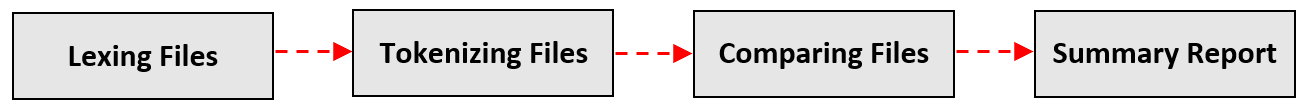
\includegraphics[scale=0.82]{ZimDesign}
\end{center}
\caption{\label{fig:design}The phases of the Zim tool.}
\end{figure}

We decided that an HTML format for the report would be best as it could be easily navigated by the user and they would only have to store the reports they're interested in, such as when the tool detects plagiarism the user would like to keep a record of. To aid in detecting plagiarism, we wanted the report to provide the file paths, an indication of the length of each match and a side by side comparison of any sections of code where a match was detected, which would allow the user to easily inspect the code and determine whether actual plagiarism has occured.

\section{Implementation}

In this section we present how the phases of Zim were implemented, outling the modules that were developed to perform the tasks discussed during the design. The module hierarchy for the implementation of Zim can be seen in figure~\ref{fig:implementation}.

\begin{figure}
\begin{center}
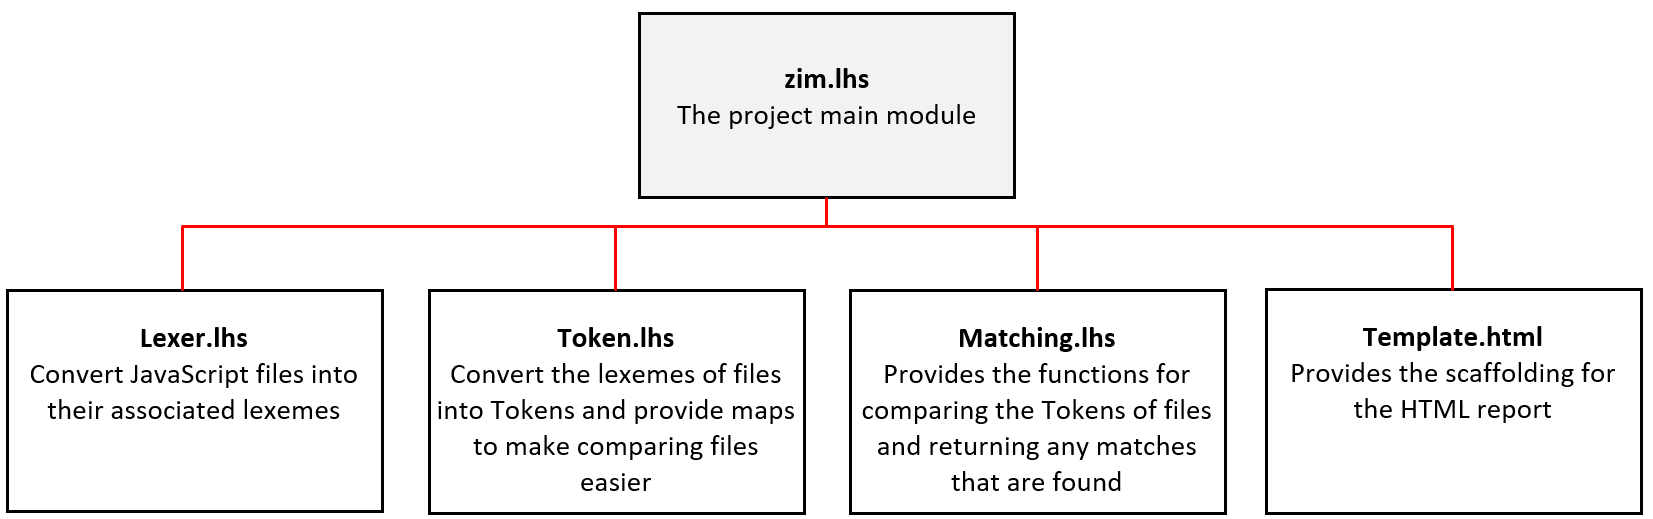
\includegraphics[scale=0.74]{ZimImplementationSummary}
\end{center}
\caption{\label{fig:implementation}The module hierarchy of Zim.}
\end{figure}

\input{zim.lhs}

\input{Zimm/Lexer.lhs}

\input{Zimm/Token.lhs}

\input{Zimm/Matching.lhs}

\subsection{template.html}

The template.html file is used to provide the scaffolding for the HTML report that summarises the results of compared files, which was achieved through utilizing the ABR.Text.Markup and ABR.Text.Configs libraries \cite{ABRLibraries}.

\bigskip

\subsection{Zim Installation}
In order to install Zim on your machine, please follow these steps:

\begin{enumerate}
	\item Download the Zim package files on your local machine.
	\item Install the most recent Glasgow Haskell Compiler (GHC) on your system, which includes cabal.
	\item Install the System.FilePath.Glob package on your system using the command {\tt cabal install glob}.
	\item Enter the zim/src directory within your local shell console and enter the command {\tt make}. This will compile all the modules required to use {\tt Zim}.
\end{enumerate}

\subsection{Zim User Guide}

Before attempting to use Zim, please ensure all modules have been compiled (see Zim Installation).

\subsubsection{Command Syntax}
To use Zim to compare files, navigate to the zim/src directory and use the following command structure within your shell console:

\bigskip

{\tt zim [-run \textless run length\textgreater ] [\textless+-\textgreater desc] [-lang \textless language\textgreater] \textless filepaths\textgreater}

\bigskip

\noindent where [ ] indicate options / flags and \textless\textgreater\hspace{0.1cm} denotes user input. 
\\
\\
Command Options / Flags:

\begin{enumerate}
	\item {\tt run <run length>} -- option used to determine the required minimum length of consecutive matching tokens before it is considered a matching run. The default value is 20.
	\item {\tt +desc} -- flag which will order the matches table of the HTML report in descending order according to the number of tokens which matched between the files. This is the default for the desc flag.
	\item {\tt -desc} -- flag which will order the matches table of the HTML report in the order that they were detected by Zim.
	\item {\tt lang <language>} -- option used to determine the programming language which will be used as the basis for comparison. The default value is JavaScript (currently the only language supported). 
\end{enumerate}

\noindent Note that all input files should match the programming language indicated, otherwise it will cause a mismatch between the elements of the language and those of the files compared, resulting in ineffective comparisons between files.

\subsubsection{Example Commands: }

\noindent {\tt zim -run 50 -desc -lang JavaScript files/*.js}
\\
\\
Compares all JavaScript files within the files/ directory (relative to current directory), using a run length of 50 (meaning atleast 50 consecutive tokens are required to match), ordering the matches table of the HTML report in descending order of matching tokens and using the JavaScript programming language as the basis for comparison.

\bigskip

\noindent {\tt zim dir1/file1.js dir2/file2.js dir3/file3.js}
\\
\\
Compares 3 JavaScript files, using a run length of 20, the JavaScript programming language as the basis for comparison, and ordering the matches table of the HTML report in descending order of matching tokens (all default values for the options / flags).

\section{Results}

In this section we will present the results of the completed Zim tool, providing examples of the tool being used to detect similiarities between files, and providing the results of the testing we performed to determine the performance of the tool.

\subsection{Function}

To test the functionality of Zim, we compared 4 files using the Zim tool to detect similarities between them. The results of the matches found between the files are provided within the HTML report and are discussed in the subsections below. 

\subsubsection{Listing the Files}

The first section of the HTML report presents: a number which maps each of the file paths to an index; the total number of tokens contained within each file; and the file paths read in by the tool. The indices provide a reference to each file, which are linked to throughout the later sections of the report and will navigate the user back to the associated file when clicked. See figure~\ref{fig:reportFiles}.

\begin{figure}
\begin{center}
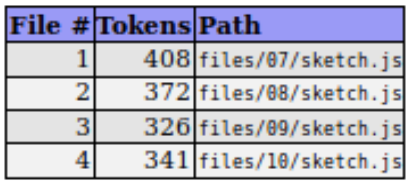
\includegraphics[scale=0.86]{ReportFiles}
\end{center}
\caption{\label{fig:reportFiles}A sample list of input files which have been compared by Zim which are presented within the HTML report.}
\end{figure}

\subsubsection{Matches}

The Matches section of the HTML report presents the matches found between the files compared, providing: the indexes for the files where each match was found; the positions in each file where the start of the matching run occurs; the length of matching tokens for each match; and an index for each match that was found, which can be clicked on to view the source code and tokens between the files that were compared. An example of the Matches table can be seen in figure~\ref{fig:reportMatches}.

\begin{figure}
\begin{center}
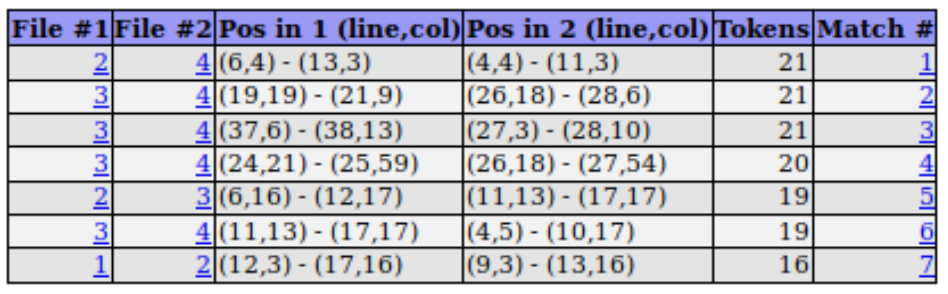
\includegraphics[scale=0.86]{ReportMatches}
\end{center}
\caption{\label{fig:reportMatches}A sample list of matches found between files compared by Zim which are presented within the HTML report.}
\end{figure}

\subsubsection{Sources}

The Sources section of the HTML report presents the sections of source code and tokens for both files where a matching run occured, presented as a side by side comparison. This allows easy inspection of the matches to determine whether actual plagiarism between the files has occured. The token side by side comparison shows the source code reconstructed from the tokenized stream of TLPs (which ignores comments and unnecessary whitspace), whereas the source code side by side comparison provides the raw source code with all comments and whitespace left intact. An example of the token comparison for a match can be seen in figure~\ref{fig:reportTokens} and the source code comparison can be seen in figure~\ref{fig:reportSources}.

\begin{figure}
\begin{center}
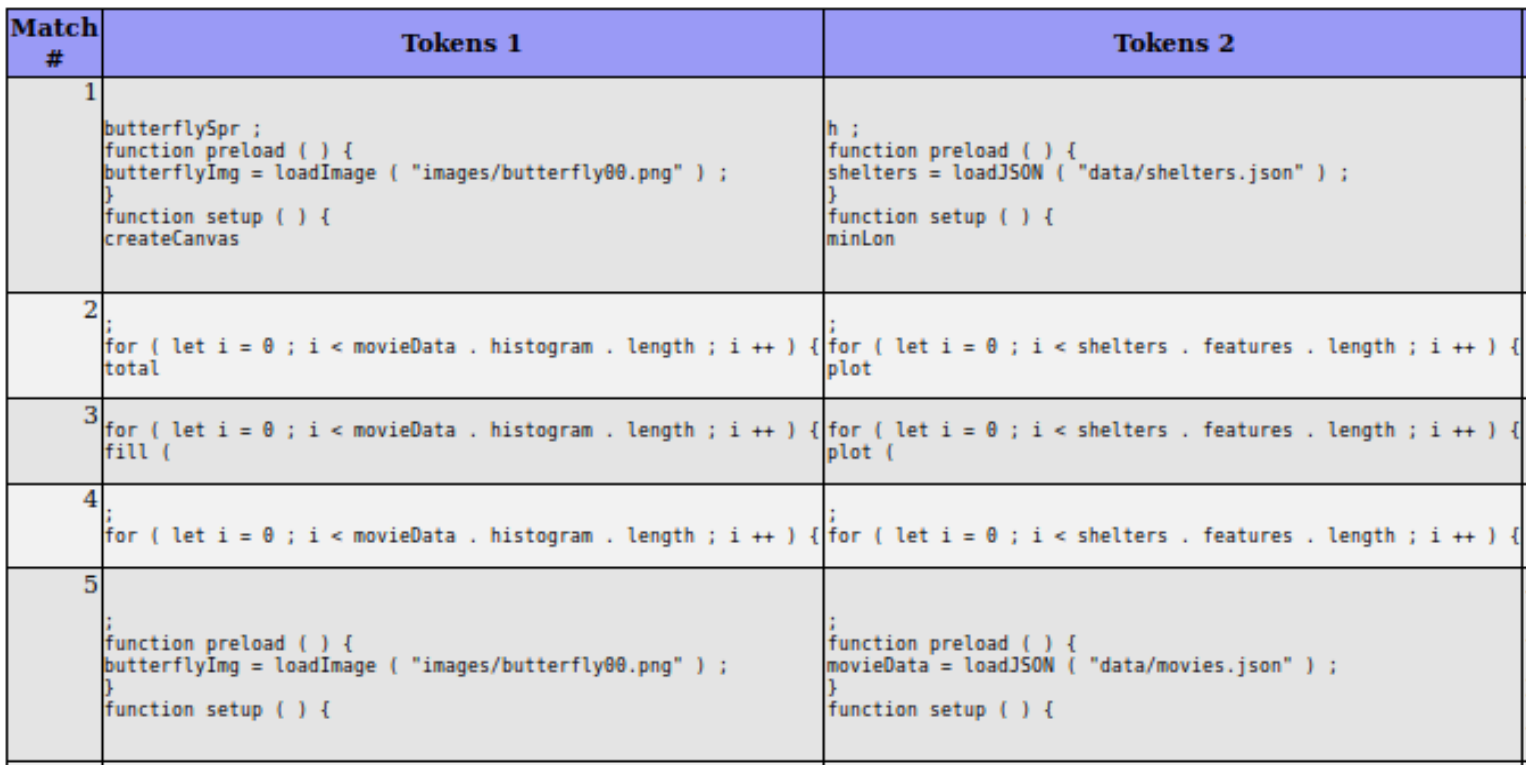
\includegraphics[scale=0.8]{ReportTokens}
\end{center}
\caption{\label{fig:reportTokens}A sample of the token comparison for matching runs found between files which are presented within the HTML report.}
\end{figure}

\begin{figure}
\begin{center}
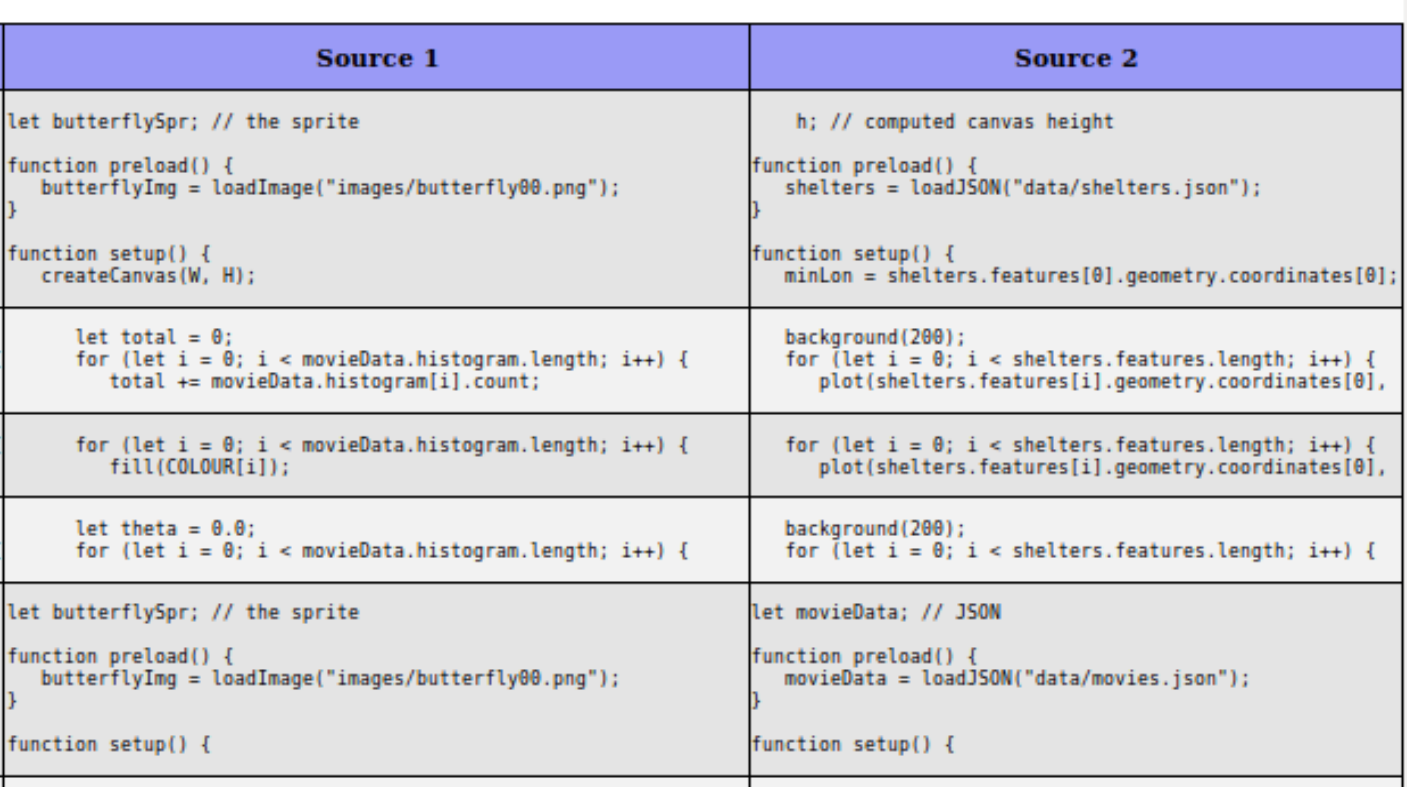
\includegraphics[scale=0.86]{ReportSources}
\end{center}
\caption{\label{fig:reportSources}A sample of the source code comparison for matching runs found between files which are presented within the HTML report.}
\end{figure}

\subsubsection{Cross Totals}

The Cross Totals section of the HTML report presents the total length of matching runs that were found between each of the compared files (for files where at least 1 matching run occured), providing a quick indication of the files which have the more severe cases of matching runs. An example of the Cross Totals can be seen in figure~\ref{fig:reportCrossTotals}.

\begin{figure}
\begin{center}
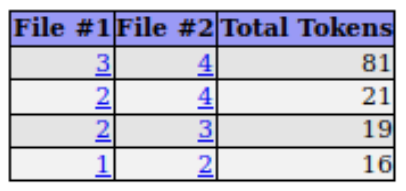
\includegraphics[scale=0.86]{ReportCrossTotals}
\end{center}
\caption{\label{fig:reportCrossTotals}A sample of the Cross Totals   which presents the total length of matching runs found between files and are presented within the HTML report.}
\end{figure}

\subsubsection{Clusters}

The Clusters section of the HTML report presents the groups of files where content may have been shared. Clusters are determined on the basis of transitivity, meaning that if file 1 has matches with file 2 and file 2 has matches with file 3, a cluster (1,2,3) is formed. For our example which compared 4 files, all of the compared files resulted in a cluster. See figure~\ref{fig:reportClusters}.

\begin{figure}
\begin{center}
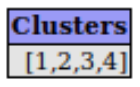
\includegraphics[scale=0.86]{ReportClusters}
\end{center}
\caption{\label{fig:reportClusters}A sample of the Clusters table which presents groups of files which share similiarities on the basis of transitivity and are presented within the HTML report.}
\end{figure}

\subsection{Performance}

To collect result for the performance of the Zim tool, we tested Zim with different numbers of files and recorded the elapsed time it took to compare all the files. This allowed us to analyse how an increasing number of files impacts the performance of the program. The raw results for the benchmarking tests can be seen in table~\ref{tab:bench} and figure~\ref{fig:bench}.

The results for these tests show that the algorithm used by Zim is quadratic with a complexity of \begin{math}O(N^2)\end{math} (where N is the number of compared files), which was determined through acquiring a slope of 1.99 when comparing the logarithms of the raw results. See figure~\ref{fig:log}.

\begin{table}
\caption{\label{tab:bench}Benchmarking results for increasing numbers of files.}
\begin{center}
\begin{tabular}{|c|c|c|} \hline
Files & Elapsed Time & Average File Size\\
(number) & (seconds) & (tokens)\\

\hline
2 & 22 & 4739\\
5 & 151 & 4012\\
10 & 491 & 3391\\
20 & 2286 & 3391\\
\hline
\end{tabular}
\end{center}
\end{table}

\bigskip

\begin{figure}
\begin{center}
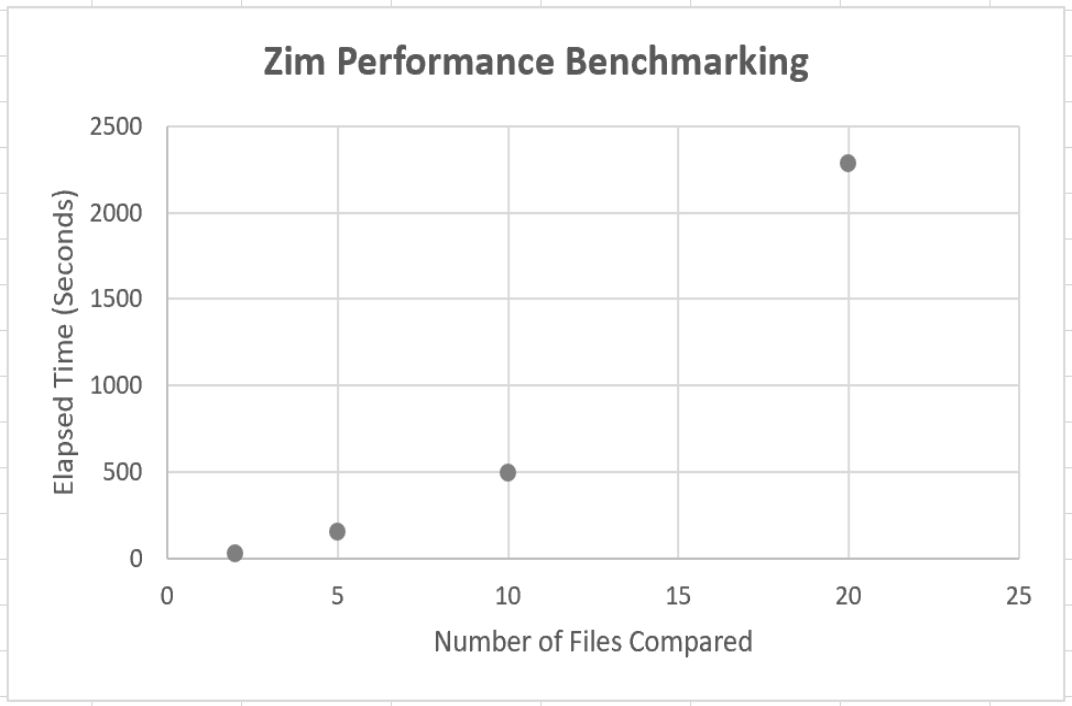
\includegraphics[scale=0.42]{ZimPerformance}
\end{center}
\caption{\label{fig:bench}Benchmarking results for increasing numbers of files.}
\end{figure}

\begin{figure}
\begin{center}
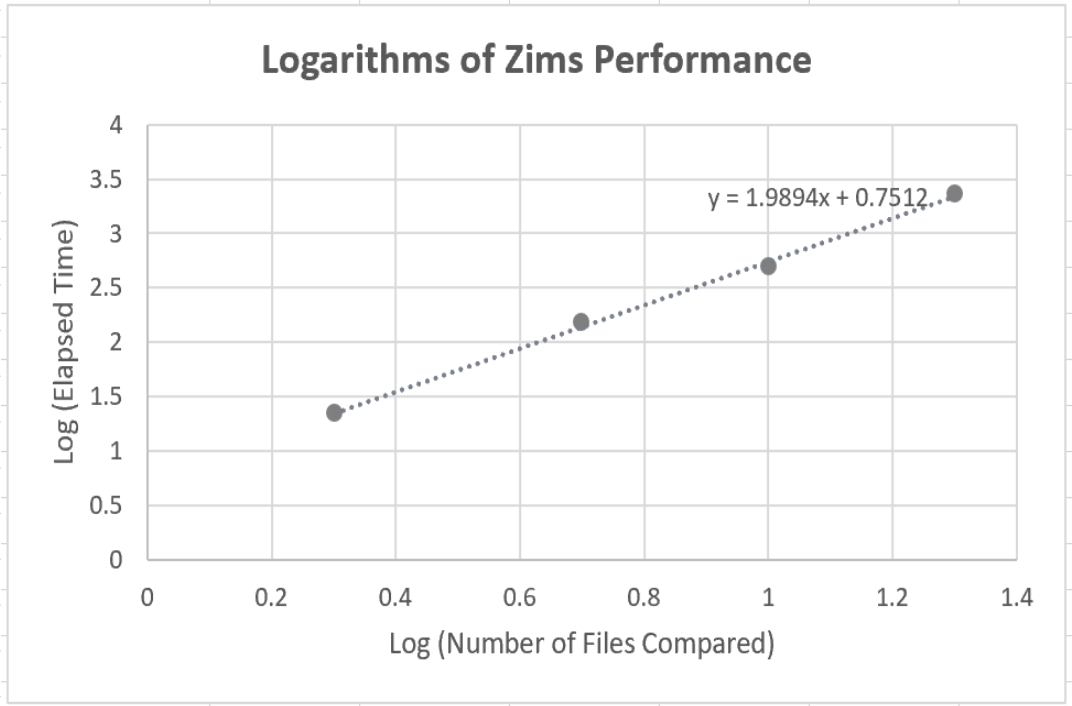
\includegraphics[scale=0.42]{ZimLog}
\end{center}
\caption{\label{fig:log}Logarithms of the Zim benchmarking results.}
\end{figure}

\section{Conclusion and Reflections}

\subsection{Discussion}
With regards to the project, Zim is successfully able to detect similarities between files and provides a conclusive summary of the results within the HTML report, which has proven to be an effective aid for detecting plagiarism. The asymptotic performance for the algorithm used in Zim ended up being quadratic with a complexity of \begin{math}O(N^2)\end{math}, which was the expected result based on our project following a similar algorithm to the Sim tool (which was also quadratic) \cite{techReport}. 

The core requirements for the project were completed in addition to a few extras to help aid in the detection of plagiarism, such as the option to order the matches of the HTML report according to the number of tokens that matched, the Cross Totals for identifying the total length of matches found between similar files, and the Cluster table to identify groups of files which are connected through similarities between them. 

\subsection{Future Work}
The Zim tool was developed with the potential for future expansion into further programming languages. In order for a new language to be added to the tool, an additional Lexer module will be required to translate files from the associated language into its lexemes. The new Lexer module should then allow for files of the new language to be lexed and tokenized, which can then be compared by the Zim tool.

The Zim tool can also be improved to make the algorithm compare files faster, as the current algorithm finds redundant matches (matches where the start and end positions are encapsulated within a previously discovered match) before discarding redundant matches once all the matches for a pair of files have been found. The algorithm would perform faster through being able to skip redundant matches during the comparison, rather then finding them then having to discard them later. 

Lastly, we believe the algorithm used for detecting clusters of plagiarised files could be further improved in the future. Currently Zim detects clusters based on transitivity, meaning that if file 1 has matches with file 2 and file 2 has matches with file 3, they form a cluster (1,2,3). However this method doesn't take into account the sections of code that matched. Even though this method is still definitely useful for detecting groups of students who share work amongst each other, we believe the algorithm could be further expanded to detect clusters when the \emph{matches} of tokens between files are similar,  which would be an effective way to detect cases where a section of code is copied amongst several files, which is a common case amongst plagiarising students. 

\subsection{Reflection}
Heading into the Functional Programming Course at the start of the trimester, I was only really expecting to learn a new 'skill' that I could apply within my programming career (how to code using functional programming languages), but I actually ended up learning more then I could have ever anticipated.

I was able to learn functional programming, how to write makefiles, and LaTeX documents, but my most significant takeaway from the course was the profound impact it had on my perspective towards different programming concepts and paradigms, which I am confident have significantly improved my capabilities as a programmer.

Programming in Haskell really helped me to understand the pitfalls of Object Oriented Programming languages, in particular, how bugs and defects are introduced into Object Oriented programs through the use of shared mutable state (entities which can change their value during runtime) and how shared mutable state makes it difficult to follow large sections of code (due to difficulty tracking the state of an entity). Furthermore, the use of shared mutable state frequently tends to make it very difficult to maintain large libraries of code, which can often lead to code having to be completely rewritten when bugs are introduced or when modifications are required.

Understanding the impact of shared mutable state has greatly improved the way I design and write code in Object Oriented languages, as I am now constantly mindful of how the code I write may impact external programs, which leads me to writing code that is better encapsulated, more predictable, easier to follow and easier to modify. 

Another significant benefit I gained from the course was the impact it had on my perspective towards writing functions. Haskell has a distinct way of incentivising \emph{small} functions (as opposed to large functions that perform a large amount of operations). Although I had to adjust initially (as I was used to writing large functions), after a while writing small functions became \emph{natural}. Now when thinking about a problem, I find myself mentally breaking it down into smaller functions / sub-problems, which has made writing code and solving problems a lot easier. Furthermore, after I had been writing small functions in Haskell for a while, I began to notice and really appreciate just how robust and reusable the code I was writing was.

Going through the course also helped me to gain a much better understanding of all the concepts and paradigms of functional programming and how to utilize them effectively. In particular, higher order functions, pattern matching, immutable state, predicates, list comprehensions, recursion, lambda functions, auxiliary functions, auxiliary expressions, referential transparency, monads, functors and lastly what I call 'pipelines' (transforming an input through piping it through multiple functions to acquire the desired result).

I feel Haskell was a key aspect of the course as it is a \emph{pure} functional programming language (meaning that it enforces the use of functional paradigms). Past courses introduced a handful of functional programming concepts, but I feel were not taught effectively due to the courses using multi-paradigm languages such as Swift or Python, which meant I could easily revert to Object Oriented style programming whenever I wanted. Not having this option in Haskell forced me to break out of that comfort zone and practice the functional programming paradigms, which contributed significantly to my learning and personal growth.

Haskell is also a very strict language, with a lot of rules being enforced by the compiler. During the early stages of the course this was difficult to deal with, mainly because the compiler would often complain about issues surrounding concepts that I had not yet been taught (such as pattern matching), which in turn made it difficult to address or understand these issues within my code. But as I became familiar with the concepts, not only did these issues become easier to address but I began to appreciate the strictness of the language and how useful this was as a tool for writing good code, where the only errors I would come across were of my own doing and not a fault of the language. 

My biggest personal difficulty with the course was when Monads were introduced, where reading up on the concept / listening to people trying to explain it didn't seem to help - but as I began to write more and more code the concept finally started to make sense.

Even though the aforementioned challenges naturally presented a very large learning curve for me, I can now fully appreciate how necessary they were for me to gain the growth I was able to achieve throughout the course.

Lastly, I was really pleased that the Zim project was completed to a standard where it could be used to achieve a useful purpose (detecting plagiarism), and was not just a 'gimmick' designed for learning purposes. I feel projects like this provide me with better preparation for post-graduate work in the IT industry, as they give a more realistic expectation of the type of work I could be asked to undertake (i.e products which are intended to be used by a customer).

To summarize I feel extremely lucky and grateful to have participated in this course, where I would go so far as to say this course has offered the most value from all the courses I have participated in throughout my degree.  

\bibliography{zim}

\end{document}
